\subsection{Report binding and challenge--response verification}
To prevent a valid geometric proof from being replayed across different reports or tasks, the protocol employs the expiring challenge-response workflow shown in Figure~\ref{fig:sequence}.

An administrator configures the task, verifying key, spacetime policy, threshold, and ordered issuer roster. The gateway retains a trusted snapshot of these settings, verifies that keys and trust-domain labels are unique, and issues a random 256-bit challenge nonce $\nu$ with an expiry timestamp $e$ from its trusted clock. The vehicle and issuers derive a shared context:


\begin{equation}\label{eq:context}
c = \mathrm{OS2IP}(\mathrm{SHA256}(\mathrm{Encode}(\mathrm{ver}, T, \nu, e, \mathrm{SHA256}(R)))) \bmod q.
\end{equation}


Here $\mathrm{ver}$ is the protocol version, $T$ is the configured task, $R$ is the raw report byte sequence, $q$ is the BN254 scalar-field modulus, and $\mathrm{OS2IP}$ maps a byte sequence to an integer. Context $c$ cryptographically binds the signed evidence and proof statement to $R$ and $\nu$ without encrypting $R$. In our implementation, $\mathrm{Encode}(\cdot)$ uses a deterministic Go JSON struct with fixed field ordering, lowercase hexadecimal SHA-256 digests, and Base64-encoded public keys.

Each issuer signs the digest $m_i$ in (2) containing $c$ and its interval bounds. After collecting all roster signatures, the vehicle evaluates the four-valued decision rule and generates a zero-knowledge proof using the interval endpoints and signatures as private witness data. The gateway verifies that $\nu$ exists and remains unexpired, reconstructs the public inputs from its trusted task snapshot and received report $R$, and verifies the proof and decision code, accepting only a verified Valid outcome.

Upon successful verification, the gateway atomically marks $\nu$ as consumed within its active instance. Failed proof verifications leave an unexpired challenge open for legitimate retries.

\paragraph{Availability and task outcomes.} The current all-roster rule deliberately fails closed when an issuer is unavailable: after the collection deadline, the vehicle cannot obtain a certificate for that challenge and must request a fresh challenge and signed observations rather than silently dropping the missing issuer. A verified Valid result admits the report; an Invalid result rejects it under the configured policy. Ambiguous is returned for host-side resensing, a revised authorized task, or manual review, while Inconsistent triggers evidence-quality diagnosis and recollection. In all non-Valid cases the gateway does not accept the report. A future $n$-of-$N$ dynamic-roster extension could use authenticated subset-selection and threshold parameters, but this is not implemented or measured by the current fixed-roster prototype.

\begin{figure}[htbp]\centering
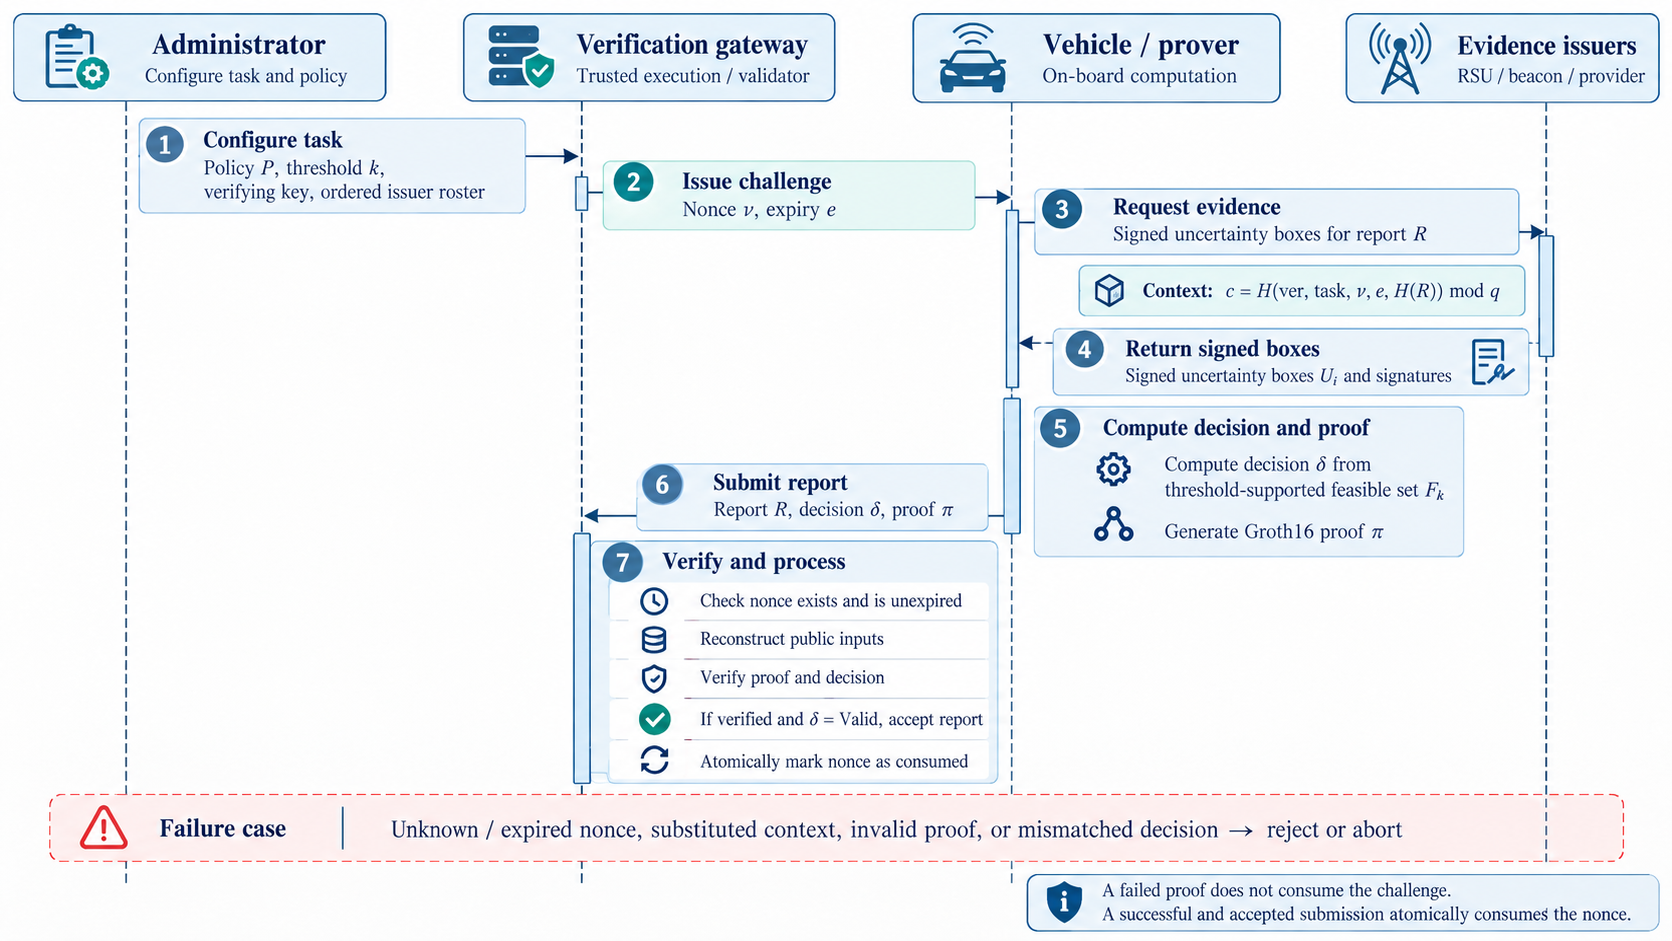
\includegraphics[width=\linewidth]{protocol_sequence.png}
\caption{Report-bound challenge-response and verification workflow. Upon successful proof verification and a Valid decision, the gateway atomically marks the nonce as consumed, whereas failed attempts leave the challenge open for retries until expiry. This schematic was generated with AI assistance (OpenAI ChatGPT); numerical and logical labels require author verification before submission.}\label{fig:sequence}
\end{figure}